\documentclass[12pt,]{article}
\usepackage{lmodern}
\usepackage{amssymb,amsmath}
\usepackage{ifxetex,ifluatex}
\usepackage{fixltx2e} % provides \textsubscript
\ifnum 0\ifxetex 1\fi\ifluatex 1\fi=0 % if pdftex
  \usepackage[T1]{fontenc}
  \usepackage[utf8]{inputenc}
\else % if luatex or xelatex
  \ifxetex
    \usepackage{mathspec}
  \else
    \usepackage{fontspec}
  \fi
  \defaultfontfeatures{Ligatures=TeX,Scale=MatchLowercase}
    \setmainfont[]{Times New Roman}
\fi
% use upquote if available, for straight quotes in verbatim environments
\IfFileExists{upquote.sty}{\usepackage{upquote}}{}
% use microtype if available
\IfFileExists{microtype.sty}{%
\usepackage{microtype}
\UseMicrotypeSet[protrusion]{basicmath} % disable protrusion for tt fonts
}{}
\usepackage[margin=2.54cm]{geometry}
\usepackage{hyperref}
\hypersetup{unicode=true,
            pdftitle={Climatic Trend Impact on Alaskan Stream Discharge},
            pdfauthor={Gaby Garcia, Walker Grimshaw, Tristen Townsend, Yixin Wen},
            pdfborder={0 0 0},
            breaklinks=true}
\urlstyle{same}  % don't use monospace font for urls
\usepackage{longtable,booktabs}
\usepackage{graphicx}
% grffile has become a legacy package: https://ctan.org/pkg/grffile
\IfFileExists{grffile.sty}{%
\usepackage{grffile}
}{}
\makeatletter
\def\maxwidth{\ifdim\Gin@nat@width>\linewidth\linewidth\else\Gin@nat@width\fi}
\def\maxheight{\ifdim\Gin@nat@height>\textheight\textheight\else\Gin@nat@height\fi}
\makeatother
% Scale images if necessary, so that they will not overflow the page
% margins by default, and it is still possible to overwrite the defaults
% using explicit options in \includegraphics[width, height, ...]{}
\setkeys{Gin}{width=\maxwidth,height=\maxheight,keepaspectratio}
\IfFileExists{parskip.sty}{%
\usepackage{parskip}
}{% else
\setlength{\parindent}{0pt}
\setlength{\parskip}{6pt plus 2pt minus 1pt}
}
\setlength{\emergencystretch}{3em}  % prevent overfull lines
\providecommand{\tightlist}{%
  \setlength{\itemsep}{0pt}\setlength{\parskip}{0pt}}
\setcounter{secnumdepth}{5}
% Redefines (sub)paragraphs to behave more like sections
\ifx\paragraph\undefined\else
\let\oldparagraph\paragraph
\renewcommand{\paragraph}[1]{\oldparagraph{#1}\mbox{}}
\fi
\ifx\subparagraph\undefined\else
\let\oldsubparagraph\subparagraph
\renewcommand{\subparagraph}[1]{\oldsubparagraph{#1}\mbox{}}
\fi

%%% Use protect on footnotes to avoid problems with footnotes in titles
\let\rmarkdownfootnote\footnote%
\def\footnote{\protect\rmarkdownfootnote}

%%% Change title format to be more compact
\usepackage{titling}

% Create subtitle command for use in maketitle
\providecommand{\subtitle}[1]{
  \posttitle{
    \begin{center}\large#1\end{center}
    }
}

\setlength{\droptitle}{-2em}

  \title{Climatic Trend Impact on Alaskan Stream Discharge}
    \pretitle{\vspace{\droptitle}\centering\huge}
  \posttitle{\par}
  \subtitle{\url{https://github.com/wgrimshaw/Alaska_DBPs.git}}
  \author{Gaby Garcia, Walker Grimshaw, Tristen Townsend, Yixin Wen}
    \preauthor{\centering\large\emph}
  \postauthor{\par}
    \date{}
    \predate{}\postdate{}
  

\begin{document}
\maketitle

\newpage

\textless{}\textbf{General Guidelines}\textgreater{} \textless{}1. Write
in scientific style\textgreater{} \textless{}2.
\href{https://rmarkdown.rstudio.com/lesson-3.html}{Global options for R
chunks} should be set so that only relevant output is
displayed\textgreater{} \textless{}3. Make sure your final knitted PDF
looks professional. Format tables appropriately, size figures
appropriately, make sure bulleted and numbered lists appear as such,
avoid awkwardly placed page breaks, etc.\textgreater{}

\hypertarget{rationale-and-research-questions}{%
\section{Rationale and Research
Questions}\label{rationale-and-research-questions}}

\textless{}Write 1-2 paragraph(s) detailing the rationale for your
study. This should include both the context of the topic as well as a
rationale for your choice of dataset (reason for location, variables,
etc.) A few citations should be included to give context for your topic.
You may choose to configure autoreferencing for your citations or add
these manually.\textgreater{}

\hypertarget{background}{%
\subsection{Background}\label{background}}

The climate is changing, in large part due to anthropogenic carbon
emissions. These changes have different magnitudes around the world and
local impacts of climate change vary as well. Specifically, climate
change is already having greater impacts near the poles than many other
parts of the globe, a process known as polar amplification or arctic
amplification (Serreze et al 2009). Understanding how climate change is
affecting discharge, especially in Alaska, has implications for water
management, ecological processes, and the larger global system (if we
consider ice-albedo feedback). Many communities rely on a given amount
of water from snowmelt to arrive at certain times of the year, so a
shift in the quantity or timing could drastically affect downstream
users and water managers. Additionally, changing the amount of flow in
rivers could affect sensitive biological communities. Furthermore,
changes in temperature that result in glacial or permafrost melting
could reduce the amount of reflective land cover, thus disrupting larger
climate systems.

\textless{}At the end of your rationale, introduce a numbered list of
your questions (or an overarching question and sub-questions). Each
question should be accompanied by one or more working hypotheses,
inserted beneath each question.\textgreater{}

\hypertarget{research-question}{%
\subsection{Research Question}\label{research-question}}

To what degree does climate change affect discharge in Alaskan streams
and rivers?

This guiding question encompasses other questions we seek to answer
through statistical analyses. If climate change is causing average
temperatures to increase, and the magnitude of the increase is greater
at higher latitudes, then higher latitude streams should demonstrate
greater changes in timing and magnitude of peak flows. This study first
seeks to examine if the magnitude of temperature changes increase with
increasing latitude in Alaska. By analyzing historical streamflow
records, we will investigate whether the magnitude of maximum daily
temperature change causes a proportional change in the magnitude and
timing of peak streamflow.

Another aspect of climate change's impacts on streamflow is the
potential of melting permafrost or glaciers. This analysis uses
cumulative annual streamflow and cumulative annual precipitation to
determine if interannual snowpack is melting with increasing average
temperatures. If so, we expect the difference between annual
precipitation and annual streamflow to increase over time.

\newpage

\hypertarget{dataset-information}{%
\section{Dataset Information}\label{dataset-information}}

\textless{}Provide information on how the dataset for this analysis were
collected, the data contained in the dataset, and any important pieces
of information that are relevant to your analyses. This section should
contain much of same information as the metadata file for the dataset
but formatted in a way that is more narrative.\textgreater{}

\hypertarget{discharge}{%
\subsection{Discharge}\label{discharge}}

Discharge data were collected from NWIS using the Data Retrieval
package. The state of Alaska was divided into 10 bins of equal latitude,
and daily discharge data was downloaded for the site in each latitude
bin with the greatest number of samples. This dataset includes the site
location, daily discharge, and county of the site, among other variables
not used in the analysis.

\hypertarget{temperature-and-precipitation}{%
\subsection{Temperature and
Precipitation}\label{temperature-and-precipitation}}

Temperature and precipitation data were downloaded from the National
Oceanic and Atmospheric Administration (NOAA) Climate Data Online web
portal. As discharge stations do not collect data on temperature and
precipitation, the climate data for each latitude bin were downloaded
from a station in the same county as each selected discharge station. In
each county, daily precipitation, maximum temperature, and minimum
temperature, data were downloaded from one station. The criteria for
station selection include data extending to the current date, beginning
at the earliest date, with at least 80\% data coverage. This dataset
also includes site location.

\textless{}Describe how your team wrangled your dataset in a format
similar to a methods section of a journal article.\textgreater{}

\newpage

\hypertarget{data-wrangling}{%
\section{Data Wrangling}\label{data-wrangling}}

\textless{}Add a table that summarizes your data structure (variables,
units, ranges and/or central tendencies, data source if multiple are
used, etc.). This table can be made in markdown text or inserted as a
\texttt{kable} function in an R chunk. If the latter, do not include the
code used to generate your table.\textgreater{}

\begin{longtable}[]{@{}rllc@{}}
\toprule
Variable & Units (if known) & Type of Variable &
Hypothesis\tabularnewline
\midrule
\endhead
Discharge & Cubic feet per second & Response & 1a, 1b, 1c\tabularnewline
Site Number & Latitude/Longitude & Predictor & 1a\tabularnewline
Date Time & Year/Month/Day & Predictor & 1c\tabularnewline
Date of First Snowmelt & Year/Month/Day & Predictor & 1a, 1b,
1c\tabularnewline
Air Temperature & Celsius & Predictor & 1b\tabularnewline
Precipitation & Millimeters & Predictor & 1a, 1c\tabularnewline
HUC 8 Watershed Size & Square Meters & Predictor & 1a, 1b\tabularnewline
Permafrost Melt & Qualitative & Predictor & 1b\tabularnewline
Glacial Coverage/Melting & Qualitative & Predictor & 1b\tabularnewline
\bottomrule
\end{longtable}

\hypertarget{data-wrangling-methods}{%
\subsection{Data Wrangling Methods}\label{data-wrangling-methods}}

(Gaby)

\hypertarget{exploratory-analysis}{%
\section{Exploratory Analysis}\label{exploratory-analysis}}

\textless{}Insert exploratory visualizations of your dataset. This may
include, but is not limited to, graphs illustrating the distributions of
variables of interest and/or maps of the spatial context of your
dataset. Format your R chunks so that graphs are displayed but code is
not displayed. Accompany these graphs with text sections that describe
the visualizations and provide context for further
analyses.\textgreater{}

\textless{}Each figure should be accompanied by a caption, and each
figure should be referenced within the text\textgreater{}

\hypertarget{snowmelt-data-wrangling}{%
\section{Snowmelt Data Wrangling}\label{snowmelt-data-wrangling}}

\hypertarget{snowmelt-graph-1}{%
\section{Snowmelt Graph 1}\label{snowmelt-graph-1}}

\begin{figure}
\centering
\includegraphics{Project_Report_v2_files/figure-latex/Snowmelt Day of Year Exploratory Graph 1-1.pdf}
\caption{Day of Year vs.~Mean Discharge. This figure shows mean
discharge across all nine latitude bins for each day of the year. This
graph served to illustrate variation across sites as to when first day
of snowmelt and peak snowmelt would occur.}
\end{figure}

\hypertarget{snowmelt-graph-2}{%
\section{Snowmelt Graph 2}\label{snowmelt-graph-2}}

\begin{figure}
\centering
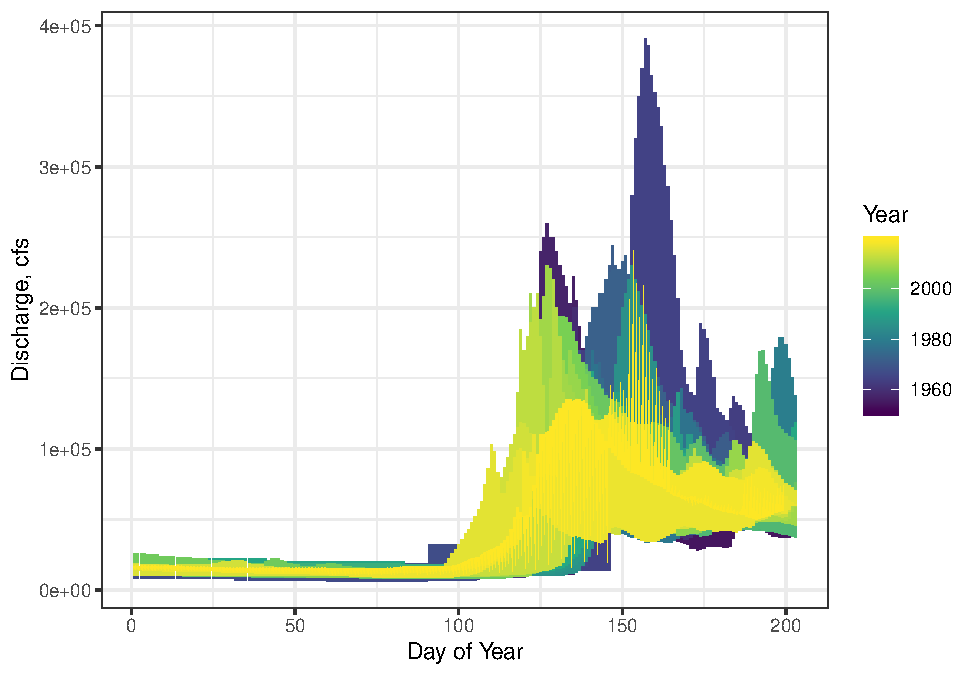
\includegraphics{Project_Report_v2_files/figure-latex/Snowmelt Day of Year Exploratory Graph 2-1.pdf}
\caption{Day of Year vs.~Discharge. This figure shows how discharge
changes with day of year across the period of record for Bin 6. This
provided a visual cue as to whether snowmelt was occuring earlier and
during what time of the year the shift was occuring.}
\end{figure}

\hypertarget{snowmelt-graph-3}{%
\section{Snowmelt Graph 3}\label{snowmelt-graph-3}}

\begin{figure}
\centering
\includegraphics{Project_Report_v2_files/figure-latex/Snowmelt Day of Year Exploratory Graph 3-1.pdf}
\caption{Day of Year vs Discharge. This figure shows how discharge
changes with day of year across the every ten years across the period of
record for fifty years. This provided a visual cue as to whether
snowmelt was occuring earlier and during what time of the year the shift
was occuring.}
\end{figure}

\hypertarget{precipitation-data-wrangling}{%
\section{Precipitation Data
Wrangling}\label{precipitation-data-wrangling}}

\hypertarget{scatterplot-of-full-precipitation-period-of-record-colored-by-bin}{%
\subsection{Scatterplot of Full Precipitation Period of Record Colored
by
Bin}\label{scatterplot-of-full-precipitation-period-of-record-colored-by-bin}}

\begin{figure}
\centering
\includegraphics{Project_Report_v2_files/figure-latex/Precipitation Exploratory Graph 1-1.pdf}
\caption{Precipitation Measured Over the Entire Period of Record by Bin.
This figure shows the general pattern of precipitation changes over
time, differentiated by the latitude bin (color). Bin 3 has the most
sample points for the entire precipitation period of record. Bin 3's
precipitation range has the greatest magnitude compared to the other
bins.}
\end{figure}

\hypertarget{group-precip-data-by-bin-and-doy-create-mean-precip-column-and-filter-weeks-to-only-include-the-spring}{%
\subsubsection{Group Precip Data by Bin and DOY, create Mean Precip
column, and filter weeks to only include the
spring}\label{group-precip-data-by-bin-and-doy-create-mean-precip-column-and-filter-weeks-to-only-include-the-spring}}

\hypertarget{graph-1}{%
\section{GRAPH 1}\label{graph-1}}

\begin{figure}
\centering
\includegraphics{Project_Report_v2_files/figure-latex/unnamed-chunk-2-1.pdf}
\caption{Day of Year vs.~Mean Precipitation. This figure shows mean
precipitation across all nine latitude bins for each day of the year.
This graph served to illustrate precipitation variation across sites.
Bin 1 has the greatest spread of mean precipitation.}
\end{figure}

\hypertarget{graph-2}{%
\section{GRAPH 2}\label{graph-2}}

\begin{figure}
\centering
\includegraphics{Project_Report_v2_files/figure-latex/unnamed-chunk-3-1.pdf}
\caption{Day of Year vs.~Precipitation. This figure shows how
precipitation changes with day of year across the period of record for
Bin 6.}
\end{figure}

\hypertarget{exploratory-precipitation-mapping}{%
\section{Exploratory Precipitation
Mapping}\label{exploratory-precipitation-mapping}}

\begin{verbatim}
## Reading layer `cb_2018_us_state_20m' from data source `/Users/gabrielagarcia/Desktop/Environmental Data Analytics/Environmental_Data_Analytics/Data/Spatial/cb_2018_us_state_20m.shp' using driver `ESRI Shapefile'
## Simple feature collection with 52 features and 9 fields
## geometry type:  MULTIPOLYGON
## dimension:      XY
## bbox:           xmin: -179.1743 ymin: 17.91377 xmax: 179.7739 ymax: 71.35256
## epsg (SRID):    4269
## proj4string:    +proj=longlat +ellps=GRS80 +towgs84=0,0,0,0,0,0,0 +no_defs
\end{verbatim}

\hypertarget{create-alaska-temp-precip-discharge-summary-using-summarize-function}{%
\section{Create Alaska Temp Precip Discharge Summary using Summarize
function}\label{create-alaska-temp-precip-discharge-summary-using-summarize-function}}

\hypertarget{noaa-site-locations-map}{%
\section{NOAA Site Locations Map}\label{noaa-site-locations-map}}

\begin{figure}
\centering
\includegraphics{Project_Report_v2_files/figure-latex/unnamed-chunk-4-1.pdf}
\caption{Map of NOAA Site Locations in Alaska}
\end{figure}

\hypertarget{mean-precipitation-map}{%
\section{Mean Precipitation Map}\label{mean-precipitation-map}}

\includegraphics{Project_Report_v2_files/figure-latex/unnamed-chunk-5-1.pdf}
\newpage

\hypertarget{mean-discharge-map}{%
\section{Mean Discharge Map}\label{mean-discharge-map}}

\includegraphics{Project_Report_v2_files/figure-latex/unnamed-chunk-6-1.pdf}
\newpage

\begin{figure}
\centering
\includegraphics{Project_Report_v2_files/figure-latex/unnamed-chunk-7-1.pdf}
\caption{Map of Mean Maximum Temperature across Alaska by Bin}
\end{figure}

\hypertarget{comparison-of-mean-precipitation-mean-discharge-and-mean-maximum-temperature-by-bin}{%
\section{Comparison of Mean Precipitation, Mean Discharge, and Mean
Maximum Temperature by
Bin}\label{comparison-of-mean-precipitation-mean-discharge-and-mean-maximum-temperature-by-bin}}

\begin{figure}
\centering
\includegraphics{Project_Report_v2_files/figure-latex/unnamed-chunk-8-1.pdf}
\caption{Comparison of Mean Precipitation, Mean Discharge, and Mean
Maximum Temperature across Alaska by Bin}
\end{figure}

\hypertarget{analysis}{%
\section{Analysis}\label{analysis}}

\textless{}Insert visualizations and text describing your main analyses.
Format your R chunks so that graphs are displayed but code and other
output is not displayed. Instead, describe the results of any
statistical tests in the main text (e.g., ``Variable x was significantly
different among y groups (ANOVA; df = 300, F = 5.55, p \textless{}
0.0001)''). Each paragraph, accompanied by one or more visualizations,
should describe the major findings and how they relate to the question
and hypotheses. Divide this section into subsections, one for each
research question.\textgreater{}

\textless{}Each figure should be accompanied by a caption, and each
figure should be referenced within the text\textgreater{}

\begin{figure}
\centering
\includegraphics{Project_Report_v2_files/figure-latex/unnamed-chunk-9-1.pdf}
\caption{Year vs.~Day of Year of Peak Discharge. This is the only
Latitude Bin with a significant change in the day of year of peak
discharge (p = 0.02353). There is a decreasing trend in the data,
indicating the day of peak snowmelt is happening sooner across
1952-2018.}
\end{figure}

\begin{verbatim}
## 
## Call:
## lm(formula = YEAR ~ DOY, data = Snowmelt.Discharge.Peaks5)
## 
## Residuals:
##     Min      1Q  Median      3Q     Max 
## -36.067 -16.464   3.743  11.960  35.689 
## 
## Coefficients:
##              Estimate Std. Error t value Pr(>|t|)    
## (Intercept) 2058.8834    31.9392  64.463   <2e-16 ***
## DOY           -0.4504     0.1942  -2.319   0.0235 *  
## ---
## Signif. codes:  0 '***' 0.001 '**' 0.01 '*' 0.05 '.' 0.1 ' ' 1
## 
## Residual standard error: 18.87 on 65 degrees of freedom
## Multiple R-squared:  0.07643,    Adjusted R-squared:  0.06222 
## F-statistic: 5.379 on 1 and 65 DF,  p-value: 0.02353
\end{verbatim}

\hypertarget{question-1}{%
\subsection{Question 1: }\label{question-1}}

\hypertarget{question-2}{%
\subsection{Question 2:}\label{question-2}}

The Climate Science Special Report estimates that maximum temperature
increases in Alaska since between the first half of the 20th century and
the past 30 years have been 1.43 degrees F
(\url{https://science2017.globalchange.gov/chapter/6/}).

\newpage

\hypertarget{summary-and-conclusions}{%
\section{Summary and Conclusions}\label{summary-and-conclusions}}

\textless{}Summarize your major findings from your analyses in a few
paragraphs. What conclusions do you draw from your findings? Relate your
findings back to the original research questions and
rationale.\textgreater{}

\newpage

\hypertarget{references}{%
\section{References}\label{references}}

 Serreze, M. C., Barrett, A. P., Stroeve, J. C., Kindig, D. N., and
Holland, M. M.: The emergence of surface-based Arctic amplification, The
Cryosphere, 3, 11--19, \url{https://doi.org/10.5194/tc-3-11-2009}, 2009.


\end{document}
